\RequirePackage{plautopatch}
\documentclass[platex, dvipdfmx]{jsarticle}
\title{浅い積雲のパラメタリゼーション}
%\date{2021.1.22}
\usepackage[dvipdfmx]{graphicx} %図の表示
\usepackage[version=3]{mhchem} %化学式
\usepackage{amsmath,here} %数式、図の位置指定

\begin{document}
\maketitle

% ___
% \_ \
%   \ \
%    \ \
%     \ \
%     _\ \_
%     \____\
\section{浅い積雲の概要}
浅い積雲は熱帯や亜熱帯で対流雲の中では最も頻度が多く,大気放射によるエネルギー収支を介して気候に与える影響が重要視されている.
浅い積雲は境界層の大気を自由大気へ輸送する役割を担っており,降水を伴わないことが多く,深い対流のように降水性の下降流が地表まで到達しないことが特徴である.

浅い積雲対流が発生する境界層の鉛直構造について簡単に説明する.地表面が太陽光によって温められた,または上方から冷たい空気が流れ込んだとき,
大気の最下層では対流不安定のエネルギーが乱流によって散逸し,海面からおよそ600mから800mの厚さで温位や水蒸気量がほぼ鉛直一様に分布する混合層を形成する.
混合層の上端には弱い安定成層の遷移層があり,ここに対流不安定による上昇流が凝結を始める高度(lifting condensation level, LCL)が位置する.
これより上では温度は湿潤断熱減率に従って変化し,上昇流は雲として観察される.さらに上昇して上向きの浮力を受けるようになる高度
(level of free convection, LFC)より上まで達する雲は周囲の空気と混合しながら成長を続ける.この対流雲の成長は自由大気下端の温度逆転層で制限され,
地表から2km程度に雲頂を持つことが多い.

% fig. 境界層の温度,湿度プロファイル

浅い積雲のパラメタリゼーションは現在気候の再現性を高めるためMIROC6から導入された.
当該のパッケージpshcn.FはPSHCNとDISTANCEのサブルーチンから成る.PSHCNの主な入力変数は気温,水蒸気量,雲水量,雲氷量である.
浅い積雲対流の鉛直輸送に応じた液水温位,総水量,雲氷量,水平風速を予報し,さらに雲量および降水量を診断する.
DISTANCEはPSHCN内部で実行され,浅い対流の浮力上昇および環境場との混合の程度を計算するものである.
様々な物理過程の中で浅い積雲が発生する条件の判定には深い対流のパラメタリゼーション(CUMULUS)で診断された変数の値を参照するため,
PSHCNおよびDISTANCEはCUMULUSの後に雲量の診断を経て実行される.また,降水を陸面や海洋のモデルで参照するため,
地表面過程(SURFCE)よりも前に実行する必要がある.

% ________
% \______ \
%   _____\ \
%   \  _____\
%    \ \    __
%     \ \___\ \
%      \_______\
\section{雲モデルの基本}

格子内の雲は主にBretherton et al. (2004)やPark and Bretherton (2009)で考案された枠組みを元にモデル化する.
このスキームではシンプルな雲のプルームモデルを採用し上昇流による保存量の鉛直輸送および降水を計算する.
一つの水平格子内の浅い積雲の集団を単一の上昇流プルームで表現し,これが周囲の環境と水平方向の混合(エントレインメント・デトレインメント)を起こすものとする.
この上昇流の鉛直輸送のフラックスを以下の形で仮定する.
\begin{equation}
    \rho \overline {w' \psi '}\approx M_u (\psi_u-\overline{\psi}) 
\end{equation}

ただし$M_u=\rho_u\sigma_u w_u$は上昇流のマスフラックス($\rho_u$,$\sigma_u$,$w_u$はそれぞれ上昇流内の密度,格子内で上昇流が占める面積比,上昇流の速度),
$\psi_u$は積雲対流で運ばれる何らかの保存量の上昇流内の代表値,$\overline{\psi}$は同じ保存量の環境場での代表値を表す.
この式における未知数$M_u$,$\psi_u$の鉛直プロファイルを求めることで浅い積雲による鉛直輸送の効果を計算する.
質量と保存量それぞれのフラックスの診断式は
\begin{align}
    \frac{\partial M_u}{\partial z} &= E - D \\
    \frac{\partial}{\partial z} (\psi_u M_u) &= X_\psi + S_\psi M_u
\end{align}

のように書ける.ただし$X_\psi$は環境場との水平方向の混合,$S_\psi$はソース項,$E$および$D$はエントレインメント割合で,

\begin{align}
    E &=\tilde{E}M_u \\
    D &=\tilde{D} M_u
\end{align}

として質量フラックスに対する比の形で記述する.$\overline{\psi}$ を格子平均値で代表させ,
水平混合の項を$X_{\psi}=E \overline{\psi} - D\psi_u$でパラメタライズすることで,上記のフラックス診断式は
\begin{align}
    \frac{\partial M_u}{\partial z} &= M_u (\tilde{E} - \tilde{D}) \\
    \frac{\partial \psi_u}{\partial z} &= \tilde{E}(\overline{\psi} - \psi_u) + S_{\psi}
\end{align}
となる.MIROC6では$S_{\psi}=0$としており,この連立方程式は$\tilde{D}$と$\tilde{E}$の二つのパラメーターについてのクロージャー問題に帰着する.
3.4節の方法で$\tilde{D}$と$\tilde{E}$を求め,雲底での境界条件とともに微分方程式を解くことで$M_u$と$\psi_u$の鉛直プロファイルを求める.

% ________
% \  ____ \
%  \_\ __\ \
%      \___ \
%     __   \ \
%     \ \___\ \
%      \_______\
\section{PSHCNでの計算}
計算手順の概略は以下の通り.

\begin{itemize}
    \item 温度$T$,比湿$q$,雲水量$l$,雲氷量$q_i$の入力から液滴温位$\theta_l$と総水量$q_t$を診断する
    \item 雲底における上昇流のマスフラックス$M_u$を診断する
    \item 雲底高度を診断する
    \item 浅い積雲の有無を診断する
    \item 上昇流内での$M_u$,$\theta_l$,$q_t$、水平風速$u$、$v$の鉛直プロファイルを診断する
    \item $\theta_l$,$q_t$,$q_i$,$u$,$v$,液滴温度$T_l$を予報する
    \item $T_l$と$q_t$から$T$,$q$,$l$を診断する
\end{itemize}


\subsection{下部境界条件:雲底での質量フラックスの診断}
雲底での質量フラックスは,境界層内部の乱流運動エネルギーと境界層上部の対流抑制(convective inhibition, CIN)に依存するように定式化する.
まず浅い積雲が存在する層全体で上昇流速の鉛直分布について
\begin{equation}
    \frac{1}{2}\frac{\partial}{\partial z}w_u^2=aB_u-b\tilde{E} w_u^2
\end{equation}
が成り立つものとする.$B_u$は上昇流内の浮力,$a,b$は経験的な定数であり,右辺第一項は浮力による加速,第二項はエントレインメントによるドラッグを意味する.
LFCより下ではエントレインメントは起こらないものと仮定し,上の式を雲底からLFCまで積分することにより,
上昇プルームが混合層からLFCまで達するための雲底での上昇流速の臨界値$w_c$が次のように求められる
\begin{equation}
    w_c = \sqrt{2a(CIN)}.
\end{equation}

この臨界値$w_c$を超えた上昇流が雲底から入ってくることになる.
CINの導出はBretherton et al. (2004) Appendix Cにならい,
\begin{align}
    CIN = [B_u(p_{base}) + B_u(p_{LCL})]\frac{p_{LCL}-p_{base}}{g(\rho_{LCL}+\rho_{base})} + B_u(p_{LCL})\frac{p_{LFC}-p_{LCL}}{g(\rho_{LFC}+\rho_{LCL})}
\end{align}
とする.以降の式でも添字$\mathit{base}$は混合層上端での値であることを示す.なおMIROC6では実装に際して
簡略化のため$B_u(p_{base})$はゼロとして計算している.

% \begin{figure}[] %位置指定はhtbp,Hで。
%     \begin{center}
%      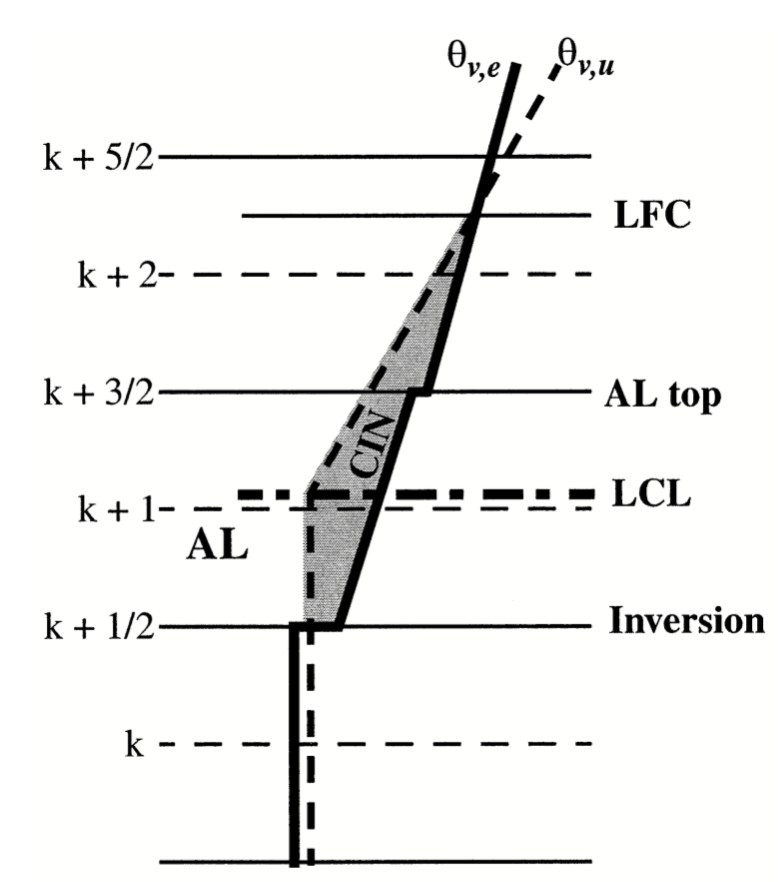
\includegraphics[width=0.4\linewidth]{fig_CIN.png}
%      \caption{上昇流内と環境場の仮温位から求めるCINの模式図.図中の``AL"は鉛直離散化の影響
%             で混合層の空気と混合層より上の空気が混ざった繊維層(ambiguous layer)を示す.
%             Bretherton et al. (2004)より引用.}
%      \label{fig_CIN}
%     \end{center}
%    \end{figure}

次に雲底での鉛直流についての情報を得るため,$w$の分布は$k_f e_{avg}$に等しい分散を持つガウス分布
\begin{equation}
    f(w) = \frac{1}{2\pi k_f e_{avg}}\exp\left[ -\frac{w^2}{2k_fe_{avg}}\right]
\end{equation}
であると仮定する.$e_{avg}$はMIROCの乱流・鉛直拡散スキームで診断された平均の乱流運動エネルギー,
$k_f$は乱流運動エネルギーが鉛直と水平の各方向に分配される比率で,LESでの検証に基づく推奨値は0.5である.
臨界値$w_c$を超える全ての範囲で上記の分布に従う上昇流速の期待値を取ることで,雲底における質量フラックス$M_{u,base}$を次のように診断する
\begin{align}
    M_{u,base}&=\overline{\rho_{base}}\int_{w_c}^{\infty}wf(w)dw \\   
    &=\overline{\rho_{base}}\sqrt{\frac{k_f e_{avg}}{2\pi}}\exp\left[-\frac{w_c^2}{2k_fe_{avg}}\right].
\end{align}
ここで$\overline{\rho_{base}}$は自由対流高度での大気の密度である.
この質量フラックスは境界層の乱流運動エネルギーが大きいほど大きく,CINが大きいほど小さくなるようになっている.

\subsection{雲底高度の診断}
雲底高度は境界層上端とLCLの間に設定することになっており,CINが大きいほど雲底が低くなる形を取る.
境界層の上端は相対湿度の鉛直勾配が最大になる高度として診断し,これとLCLとのうち高い方を$z_{Hi}$,低い方を$z_{Lo}$とすれば,雲底高度$z_{base}$は
\begin{equation}
    z_{base} = z_{Hi} - (z_{Hi}-z_{Lo})\frac{CIN-CIN_{Lo}}{CIN_{Hi} - CIN_{Lo}}    
\end{equation}
とする.ただし$CIN_{Hi}$,$CIN_{Lo}$はそれぞれCINの典型的な値に対して$CIN_{Lo}\le CIN \le CIN_{Hi}$となるような定数である.

\subsection{浅い積雲の有無の判定}
 各水平格子について,以下の条件によって浅い積雲対流が発生するかどうかを判定する.
 \begin{itemize}
    \item 推定逆転層強度(estimated nversion strength, EIS; Wood and Bretherton, 2006) がある閾値を超える場合は,層積雲が卓越する環境場であると判断し,浅い積雲は発生させない.
     この基準は,気候モデルの鉛直解像度では境界層の上にできる薄く強い逆転層を十分に表現できず,
     CINの過小評価により浅い積雲が過大に表現される問題があるため導入されている.EISは
     $EIS=\theta_{700}-\theta_{0}-\Gamma_m^{850}(z_{700}-LCL)$
    で求める.ただし$\theta_{700}$,$\theta_0$はそれぞれ700hPaと地表面での温位,$\Gamma_m^{850}$は850hPa高度の湿潤断熱減率,
    $z_{700}$は700hPa高度である.
   \item 深い積雲のスキームで診断された積雲対流の深さが特定の閾値を超えた場合,深い対流卓越する環境場であるとし,浅い積雲は発生させない.
   \item 浅い積雲に伴う上昇流の面積が或る閾値を越えない場合浅い積雲の計算を省略する. 
 \end{itemize}

\subsection{上昇流フラックスの鉛直プロファイルの診断}
浅い積雲が発生すると判定された雲底と判断された格子では,上述の雲底高度に輸送される量$\psi_u$の境界層格子平均値と雲底の質量フラックス
$M_{u,base}$を与え,エントレインメントとデトレインメントを計算していく.
エントレインメントとデトレインメントの比率$\tilde{E}$, $\tilde{D}$を決定するプロセスはKain and Fritsch (1990)などでも用いられている
浮力ソートの考え方を利用する.厚さ$\delta z$の層内で,環境場の空気$\delta M_e$と上昇流内の空気$\delta M_u$が等しく
$\tilde{E_0} M_u \delta z$ずつ水平混合に関与して様々な混合状態のスペクトルを成す状況を考える.
混合に関与する全質量フラックスは$2\tilde{E_0} M_u\delta z$である.ただし$\tilde{E_0}$は$\tilde{E_0}=c_0/H$で与えられる量で$c_0$は経験定数,$H$は対流圏の厚さである.
混合空気内では,環境場からの空気が比率$\chi$を占めるような混合状態が確率密度$q(\chi)$で存在しており,
ここでは計算を簡単にするため$\chi=0$の純粋な湿潤空気から$\chi=1$の純粋な環境場の空気までの混合状態が一様な確率で分布していると考える
(Kain-Fritschスキームではガウス分布を仮定している).この混合空気にはたらく浮力を元にエントレインメントまたはデトレインメントが判定され,
この過程でPSHCNの内部でサブルーチンDISTANCEが呼び出される.上昇流の液水温位(THETLU)とエントレインメント・デトレインメントの判定のブール値(JUDGE)が出力変数である.

% \begin{figure}[] %位置指定はhtbp,Hで。
%     \begin{center}
%      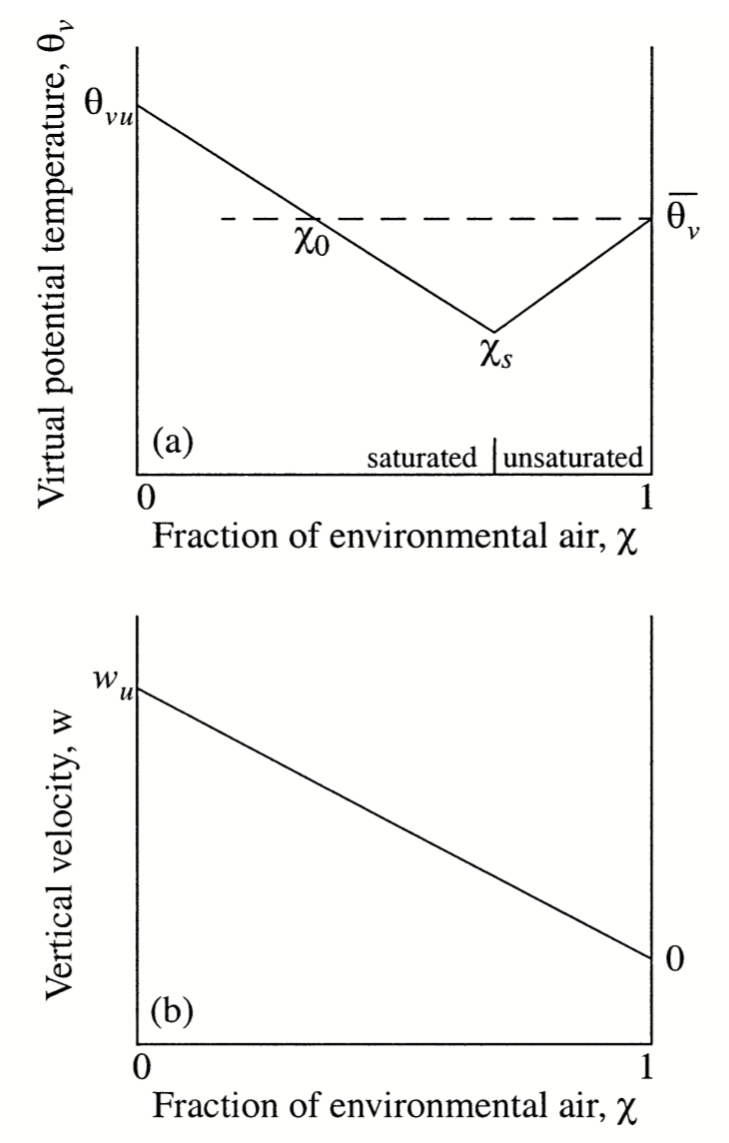
\includegraphics[width=0.4\linewidth]{fig_chi.png}
%      \caption{混合の比率$\chi$による(a)仮温位と(b)上昇流速の変化.図中$\chi_0$は浮力が0になる$\chi$の値,$\chi_s$は混合空気が飽和するときの$\chi$の値を表す.
%                 Bretherton et al. (2004)より引用.}
%      \label{fig_chi}
%     \end{center}
%    \end{figure}

エントレインメントの条件は以下のように判定される.まず上昇流が飽和しているかを判断し,飽和していなければエントレインメントは起こらない.
次にパーセルに働く浮力を環境場の仮温位$\overline{\theta_v}$,上昇流内の仮温位$\theta_{vu}$を用いて

\begin{equation}
    B_u = g\frac{\theta_{vu} - \overline{\theta_{v}}}{ \overline{\theta_v}}
\end{equation}
で計算し,正の浮力を持つ場合にはエントレインメントが起こるとする.
さらに,浮力が負の場合でも慣性によってある渦混合距離$l_c$を超えて上昇し続けることができる場合にはエントレインメントが起こるものとする.
混合距離は$l_c \equiv c_1 H$で定義する.ただし定数$c_1=0.1$は貿易風帯のケースに最適化した値を使用している.
上昇流内の浮力$B_u$が臨界値
\begin{equation}
    B_c = -\frac{1}{2}\frac{w_u^2}{l_c}    
\end{equation}
を超えていればエントレインメントが起こると判定され,それ以外の混合空気はすべてデトレインされる.
負の浮力を受けながら距離$l_c$だけ上昇できるような混合状態の臨界値$\chi_c$が求まれば,エントレインメントによって上昇流内に取り込まれる環境場の空気
\begin{equation}
    2\tilde{E_0} M_u\int_0^{\chi_c}\chi q(\chi) d\chi = \tilde{E_0} M_u \chi_c^2    
\end{equation}
とデトレインメントによって環境場へ放出される上昇流内の空気
\begin{equation}
    2\tilde{E_0} M_u\int_{\chi_c}^{1}(1-\chi) q(\chi) d\chi = \tilde{E_0} M_u (1-\chi_c)^2    
\end{equation}
が計算でき,
\begin{align}
    \tilde{E}&=\tilde{E_0}\chi_c^2 \\
    \tilde{D}&=\tilde{E_0}(1-\chi_c)^2 \\
    \frac{1}{M_u}\frac{\partial M_u}{\partial z} &= \tilde{E} - \tilde{D} = \tilde{E_0}(2\chi_c - 1) \label{M_u}\\
    \frac{\partial \psi_u}{\partial z} &= \tilde{E} (\overline{\psi}-\psi_u) = \tilde{E_0}\chi_c^2(\overline{\psi}-\psi_u) \label{psi_u}\\
\end{align}

となる.$\chi_c$は混合空気の仮温位
\begin{equation}
    \theta_v(\chi)=\theta_{vu}+\chi\left[ \beta(\overline{\theta_l}-\theta_{l,u})-\left(\frac{\beta L}{c_p\Pi}-\theta_u\right)(\overline{q_t}-q_{l,u})\right]   
\end{equation}
(Randall,1980)をもとに導出する.

$\psi_u$の中の液水温位と総水量から雲水量$l$と比湿$q$を診断し,閾値を上回った雲水は雨水$q_r$として落下させる.$q_r$の生成量に応じて液水温位を更新し,
$w_u$および$M_{u,base}$と整合するように上昇流の面積を診断する.これを離散化した支配方程式(\ref{M_u}),(\ref{psi_u})で上方に積分していくことで上昇流の鉛直プロファイルを求めていき,
$w_u$または上昇流面積が下限値の定数を下回る高さを雲頂高度とする.
なお,本パラメタリゼーションでの保存量の鉛直フラックスの定式化は,講師の下端から流入する上昇流は時間ステップ$\Delta t$で
格子内の大気を全て入れ替えるほど大きくないと仮定しているに等しい.よって上昇流の質量フラックスを求める際には次のような上限を課して数値不安定を防いでいる.
\begin{equation}
    M_u = min.\left(M_u, \frac{\rho\Delta z}{\Delta t}\right)    
\end{equation}

\begin{thebibliography}{99}
    \bibitem{B04} Bretherton, C. S., J. R. McCaa, and H. Grenier 2004: 
        A new parameterization for shallow cumulus convection and its application to marine subtropical cloud-topped boundary layers. 
        Part I: description and 1D results, \textit{Mon. Wea. Rev.}, 132, 864-882.
    \bibitem{KF90}Kain, J. S., and J. M. Fritsch 1990: 
        A one-dimensional entraining/detraining plume model and its application in convective parameterization,
        \textit{J. Atmos. Sci.}, 47, 2784-2802.
    \bibitem{PB09} Park, S. and C. S. Bretherton 2009: 
        The University of Washington shallow convection and moist turbulence schemes and their impact on 
        climate simulations with the Community Atmosphere Model, \textit{J. Clim}, 22, 3449-3469.
    \bibitem{R80} Randall, D. A. 1980: 
        Conditional instability of the first kind upside-down. \textit{J. Atmos. Sci.}, 37, 125–130.
    \bibitem{SouseiRep} Ogura, T. 2015: 
        Implementation of a shallow convection parameterization. \textit{Program for Risk Information on Climate Change, 
        Progress report 2014}, 126-131.
    \bibitem{WB06} Wood, R. and C. S. Bretherton 2006: 
        On the relationship between stratiform low cloud cover and lower-tropospheric stability. 
        \textit{J. Clim}, 19, 6425–6432.
\end{thebibliography}

\end{document}